\documentclass[10pt,letterpaper]{article}
\usepackage[margin=0.75in]{geometry}
\usepackage{amsmath}
\usepackage{amsfonts}
\usepackage{amssymb}
\usepackage{graphicx}
\usepackage{cancel}
\usepackage{listings}
\usepackage{color}
\usepackage{textcomp}
\definecolor{listinggray}{gray}{0.9}
\definecolor{lbcolor}{rgb}{0.9,0.9,0.9}
\lstset{
	backgroundcolor=\color{lbcolor},
	tabsize=4,
	rulecolor=,
	language=Python,
        basicstyle=\scriptsize,
        upquote=true,
        aboveskip={1.5\baselineskip},
        columns=fixed,
        showstringspaces=false,
        extendedchars=true,
        breaklines=true,
        prebreak = \raisebox{0ex}[0ex][0ex]{\ensuremath{\hookleftarrow}},
        frame=single,
        showtabs=false,
        showspaces=false,
        showstringspaces=false,
        identifierstyle=\ttfamily,
        keywordstyle=\color[rgb]{0,0,1},
        commentstyle=\color[rgb]{0.133,0.545,0.133},
        stringstyle=\color[rgb]{0.627,0.126,0.941},
}

\def\mbf{\mathbf}
\def\mbb{\mathbb}

\providecommand{\abs}[1]{\left\lvert#1\right\rvert}
\providecommand{\norm}[1]{\left\lVert#1\right\rVert}
\def\d{\mathrm{d}}
\def\e{\mathrm{e}}

\title{Numerical Treatment of Differential Equations: Homework 7}
\author{Truman Ellis}

\begin{document}
\maketitle

We wish to solve the second order differential equation
\begin{align*}
&-u(x)''+cu(x)=f(x)\,,\quad \text{ in } (0,1)\\
&u(0)=u_L\,,\quad\quad u(1)=u_R\,,
\end{align*}
for $c\ge0$. We will solve this with continuous first order basis functions.
This boils down to a linear system of equations
\[
\mathbf{A}\boldsymbol\alpha=\mathbf{b}\,,
\]
where 
\begin{align*}
&A_{ij}=(\phi_i',\phi_j')+(c\phi_i,\phi_j)\\
&b_i=(f,\phi_i)-u_L[(\phi_0',\phi_i')+(c\phi_0,\phi_i)]-u_R[(\phi_N',\phi_i')+(c\phi_N,\phi_i)]\,.
\end{align*}

In one dimension, we can calculate most of these integrals explicitly. For
uniform spacing, we get $(\phi_i',\phi_i')=\frac{2}{h}$,
$(\phi_i',\phi_{i\pm1}')=-\frac{1}{h}$, $(\phi_i,\phi_i)=\frac{2h}{3}$,
$(\phi_i,\phi_{i\pm1})=\frac{h}{6}$, and all other terms are zero.
Using the trapezoid rule, we can approximate $(f,\phi_i)=hf(x_i)$.

Using the method of manufactured solutions, we can test the convergence of our
method. If we wish to converge to an exact solution $u_{ex}=\sin(4\pi x^3)+5x-3$
with boundary conditions $u_L=-3$ and $u_R=2$, we can set our forcing function
to be $f(x)=-u_{ex}(x)''+cu_{ex}(x)$.

We achieve quadratic convergence in both the quasi-optimal error norm and the
$L_2$ norm as we see in the following figures. This is higher than expected for
the quasi-optimal error norm, and there are several possible explanations. With
this uniform mesh, I could be seeing a case of superconvergence. Alternatively
the solution at the half node values could be second order accurate and using
these exclusively to calculate the error integral could be artificially reducing
my error calculation. The third option is that there is a bug in the code, but
since everything else is working so well, I think one of the first two options
is more likely.

We have no issue solving with
zero or large $c$, in fact the convergence plots look nearly identical. However,
as the final three figures demonstrate, the solution degrades for negative $c$.

\begin{figure}[p]
\begin{center}
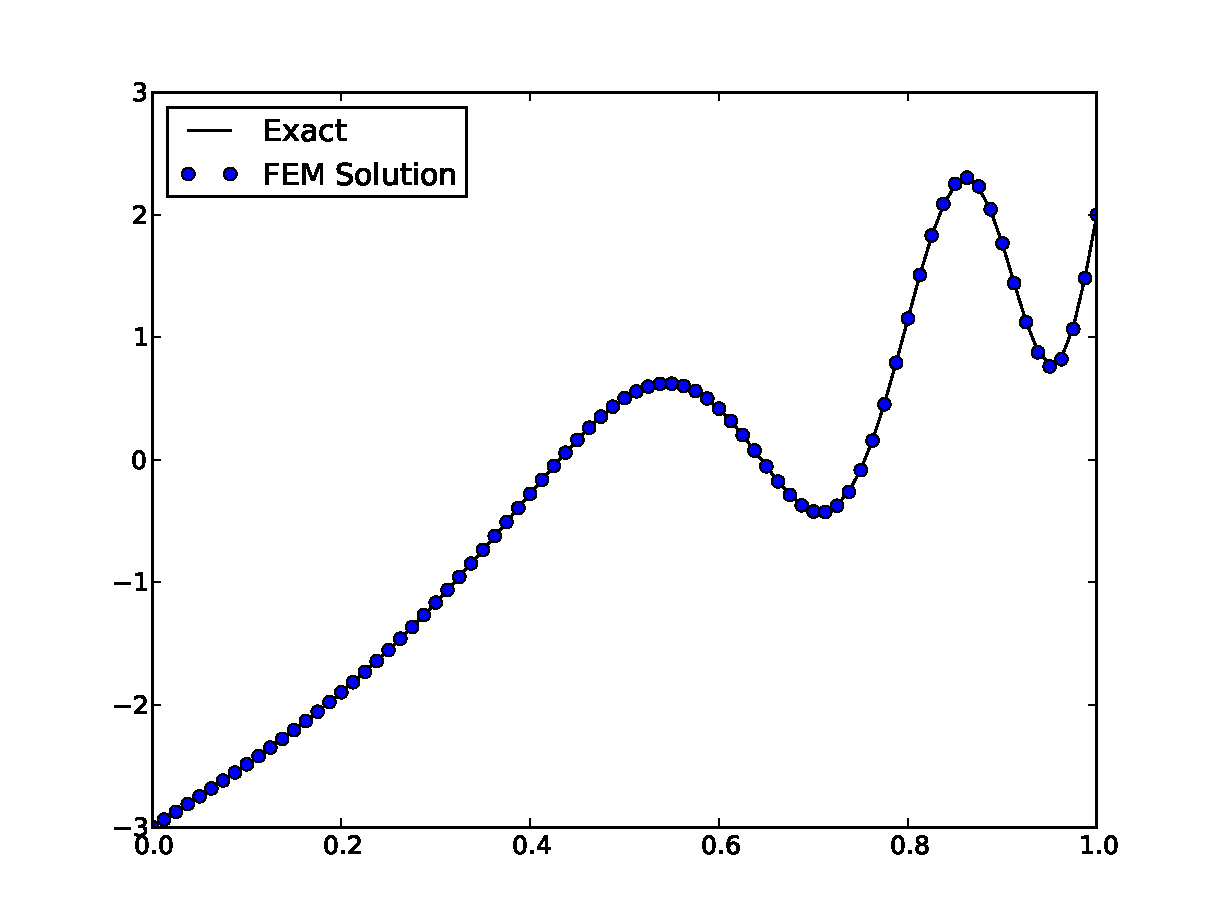
\includegraphics[width=5in]{c1.pdf}
\end{center}
\caption{Finite element vs exact solution, for $c=1$}
\label{fig:soln}
\end{figure}

\begin{figure}[p]
\begin{center}
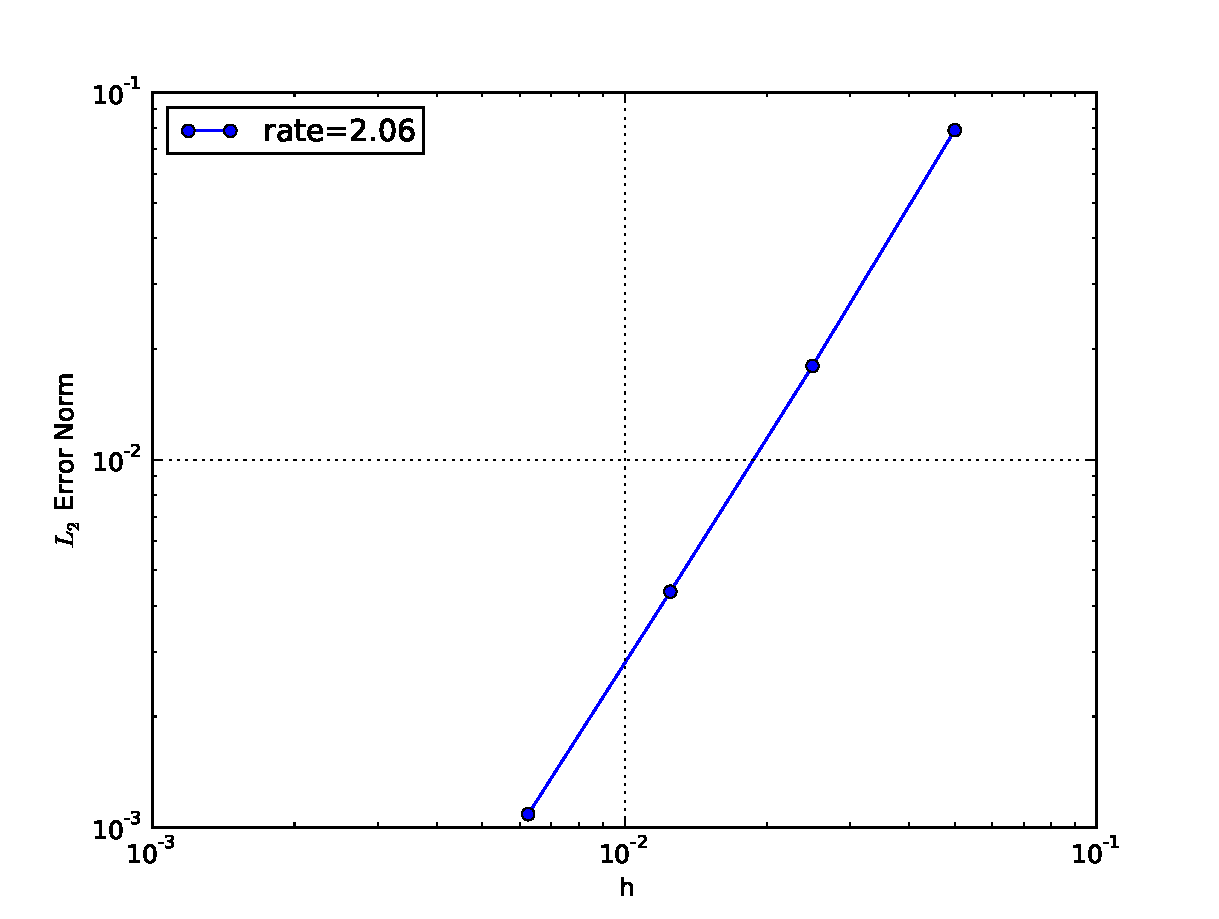
\includegraphics[width=5in]{ec1.pdf}
\end{center}
\caption{$L_2$ convergence for $c=1$}
\end{figure}

\begin{figure}[p]
\begin{center}
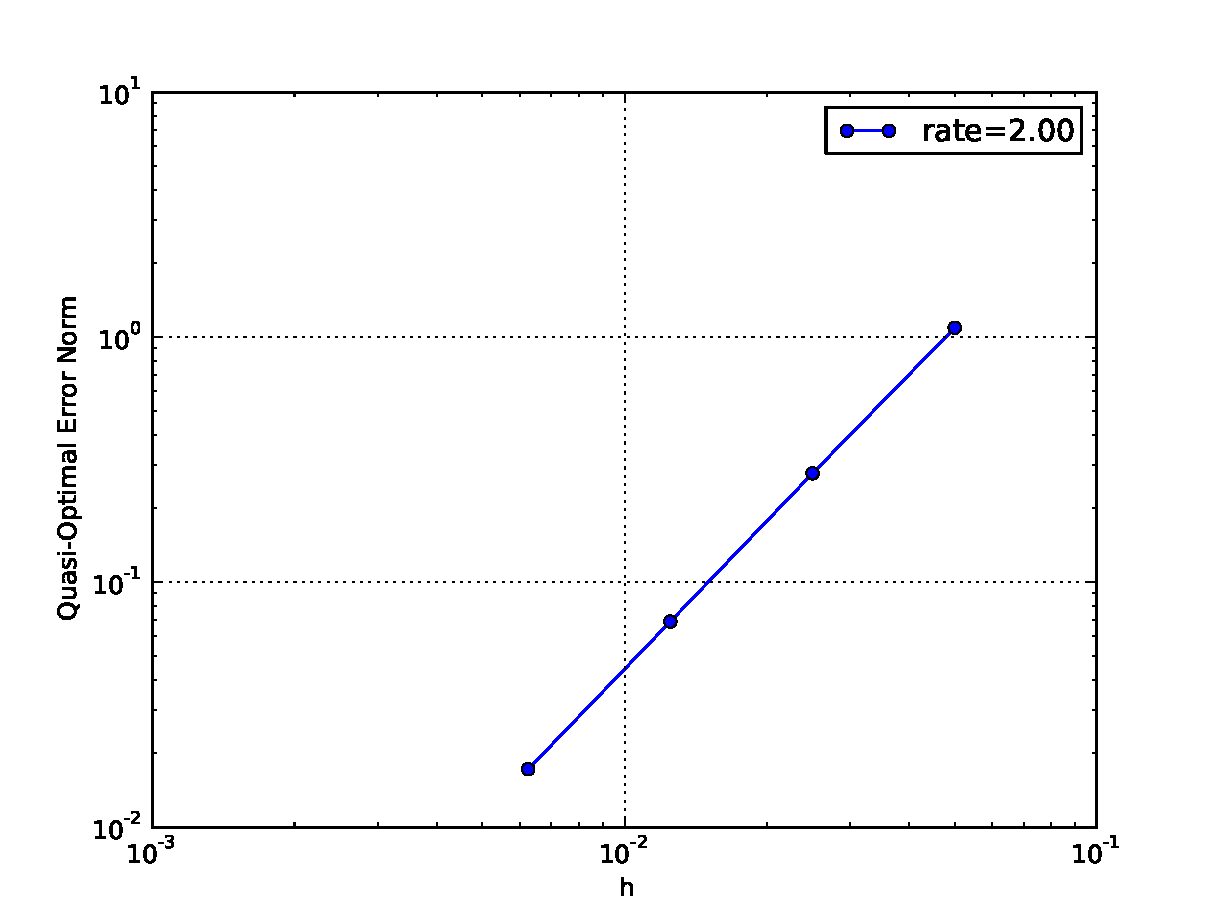
\includegraphics[width=5in]{epc1.pdf}
\end{center}
\caption{Quasi-optimal convergence for $c=1$}
\end{figure}

\begin{figure}[p]
\begin{center}
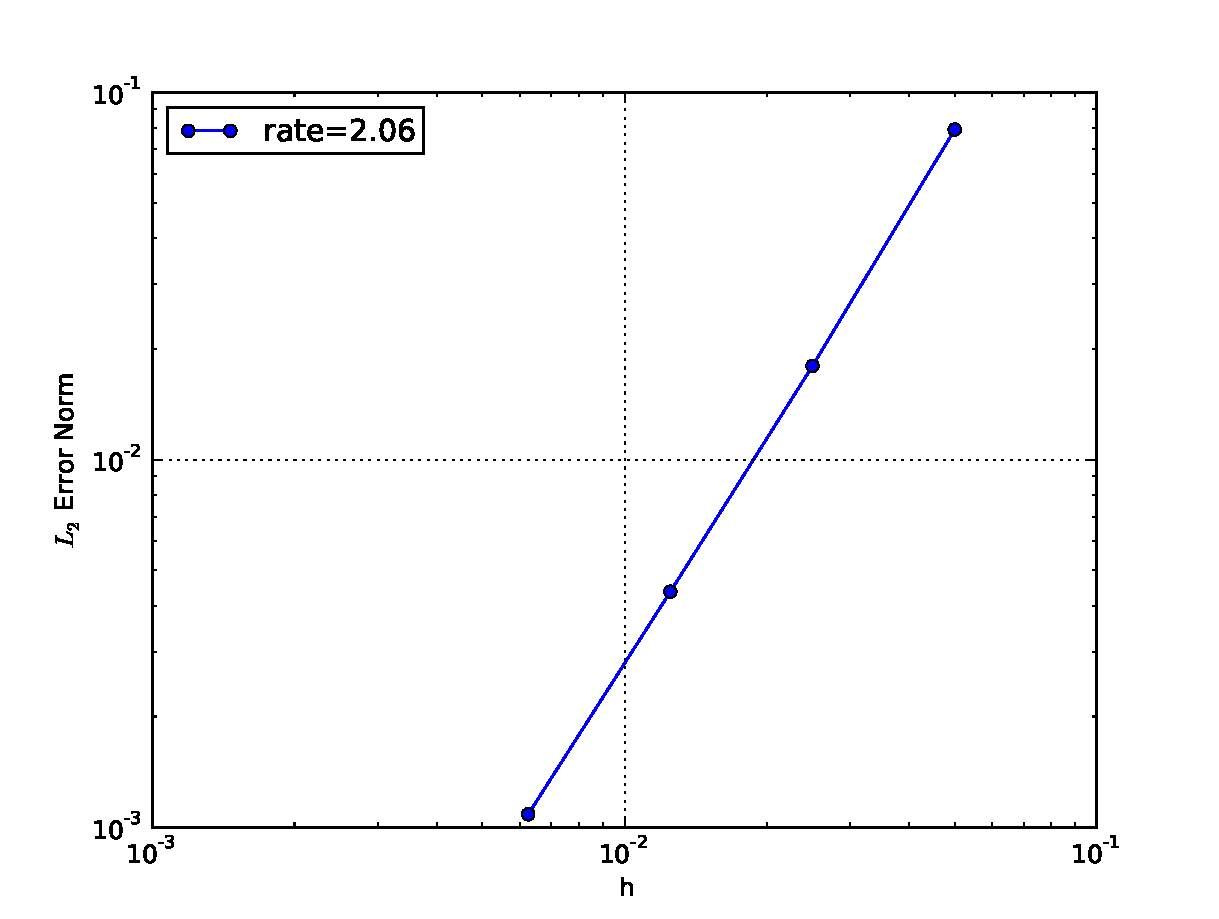
\includegraphics[width=5in]{ec0.pdf}
\end{center}
\caption{$L_2$ convergence for $c=0$}
\end{figure}

\begin{figure}[p]
\begin{center}
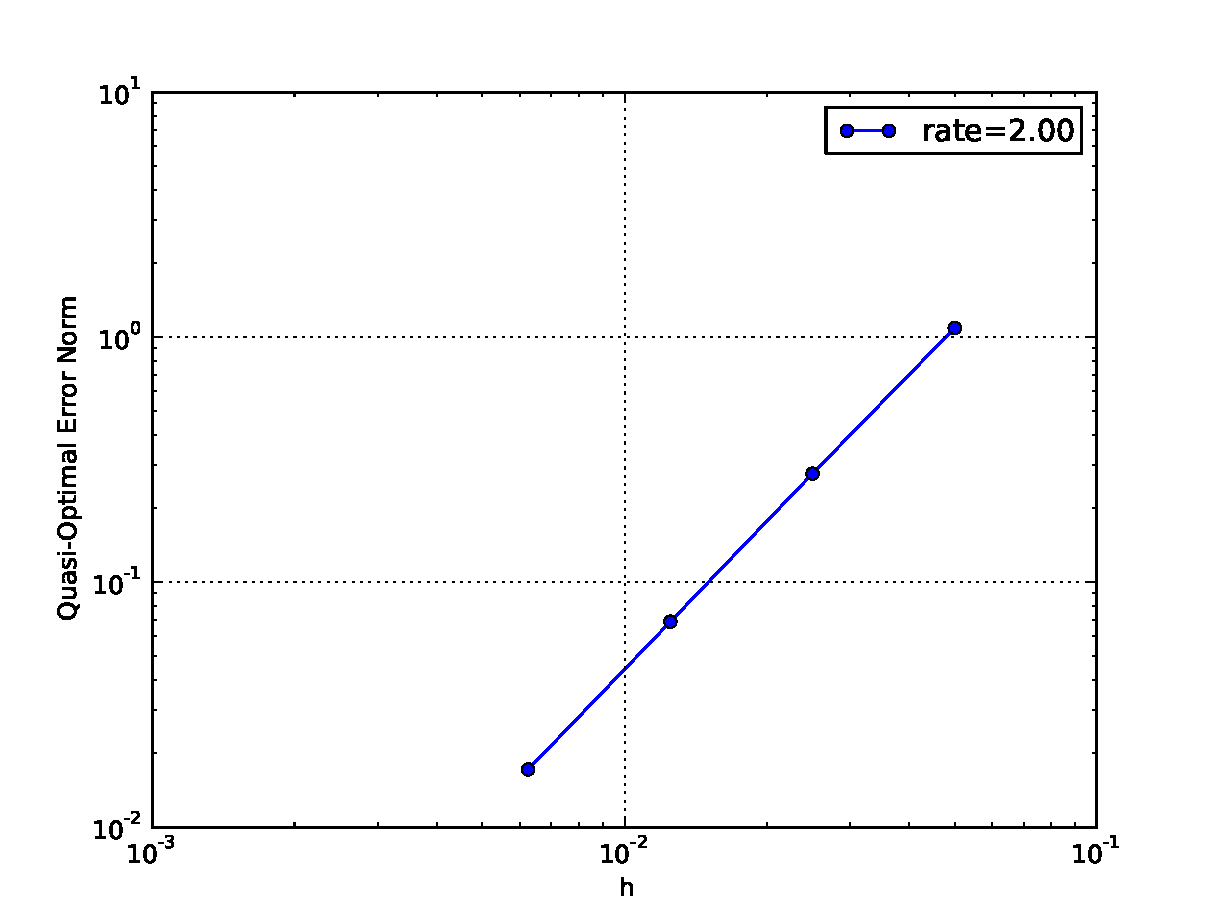
\includegraphics[width=5in]{epc0.pdf}
\end{center}
\caption{Quasi-optimal convergence for $c=0$}
\end{figure}

\begin{figure}[p]
\begin{center}
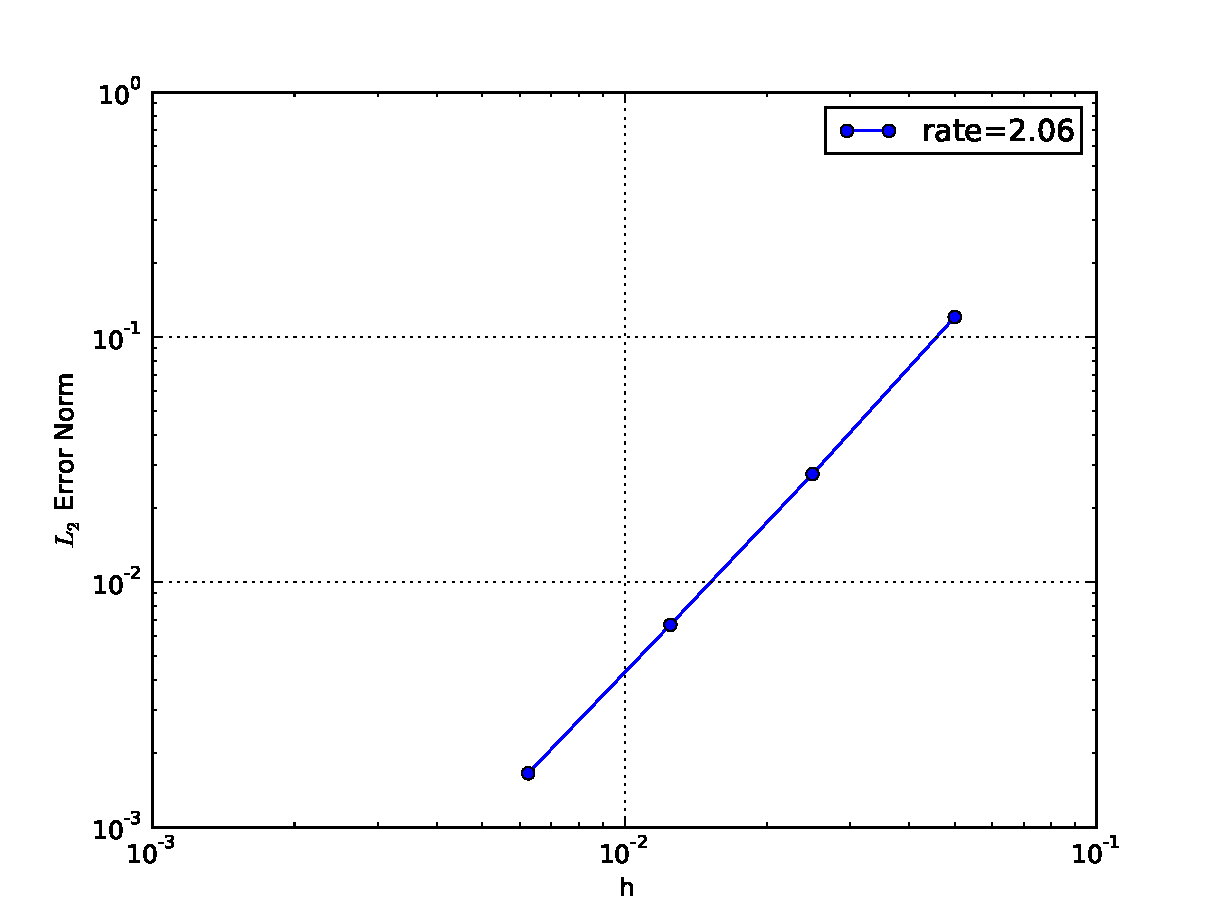
\includegraphics[width=5in]{ec1000.pdf}
\end{center}
\caption{$L_2$ convergence for $c=1000$}
\end{figure}

\begin{figure}[p]
\begin{center}
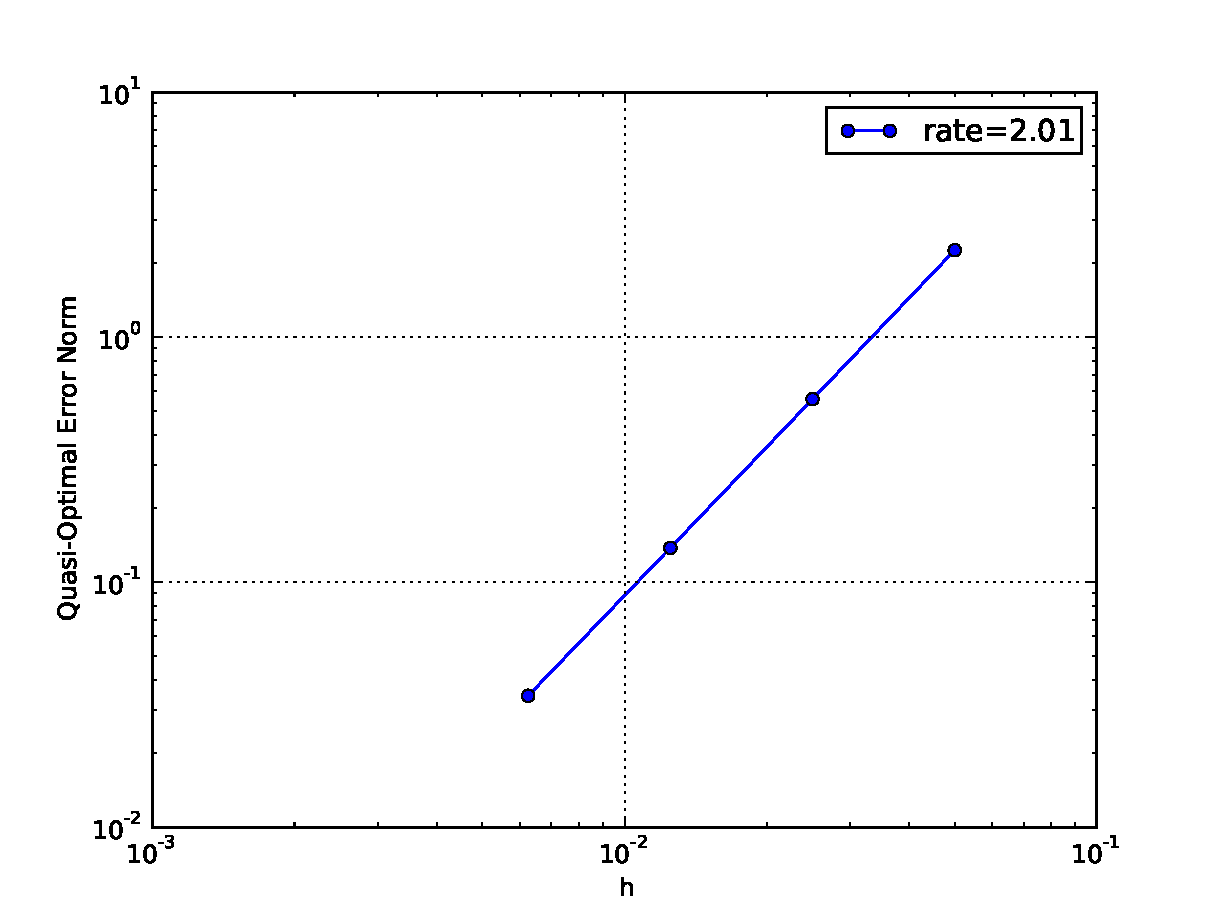
\includegraphics[width=5in]{epc1000.pdf}
\end{center}
\caption{Quasi-optimal convergence for $c=1000$}
\end{figure}

\begin{figure}[p]
\begin{center}
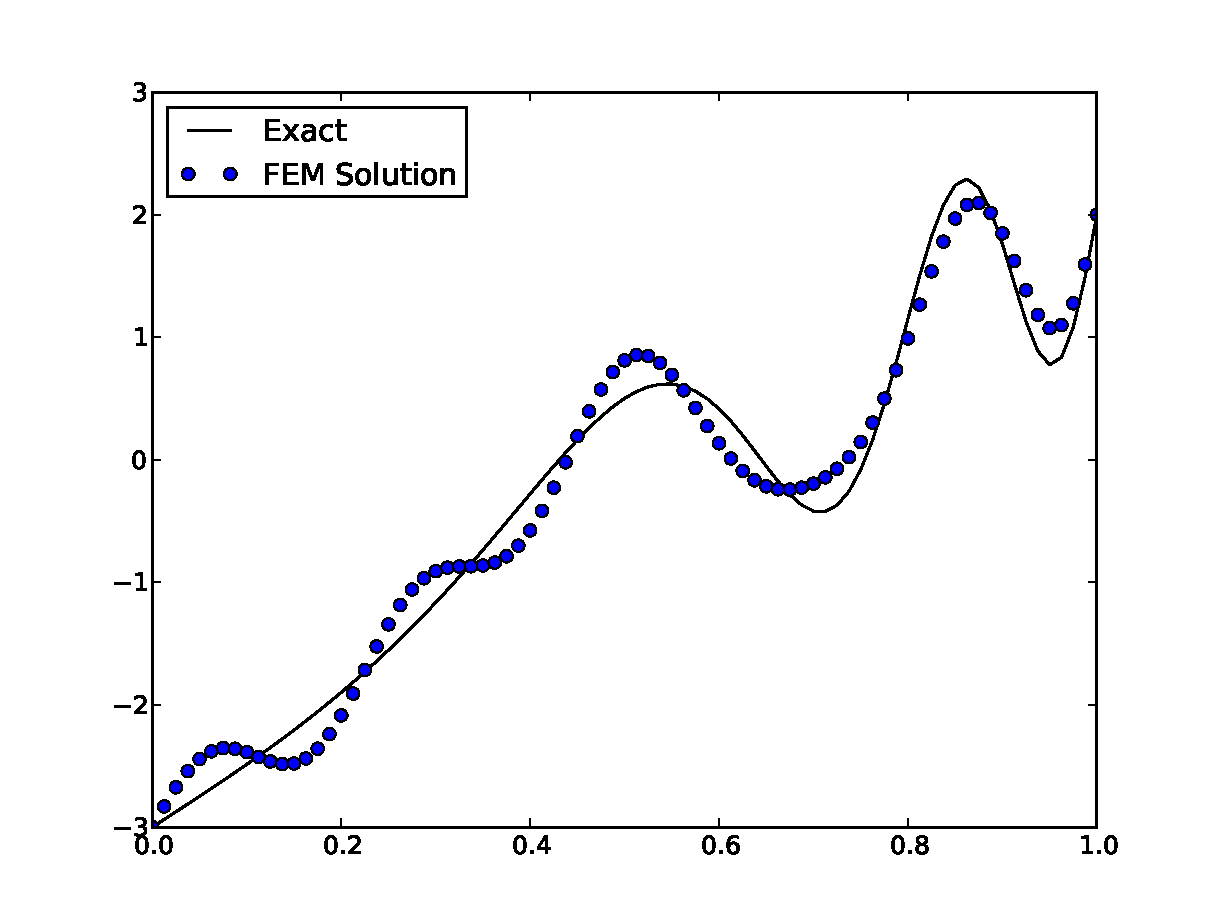
\includegraphics[width=5in]{c-800.pdf}
\end{center}
\caption{Finite element vs exact solution, for $c=-800$}
\label{fig:negsoln}
\end{figure}

\begin{figure}[p]
\begin{center}
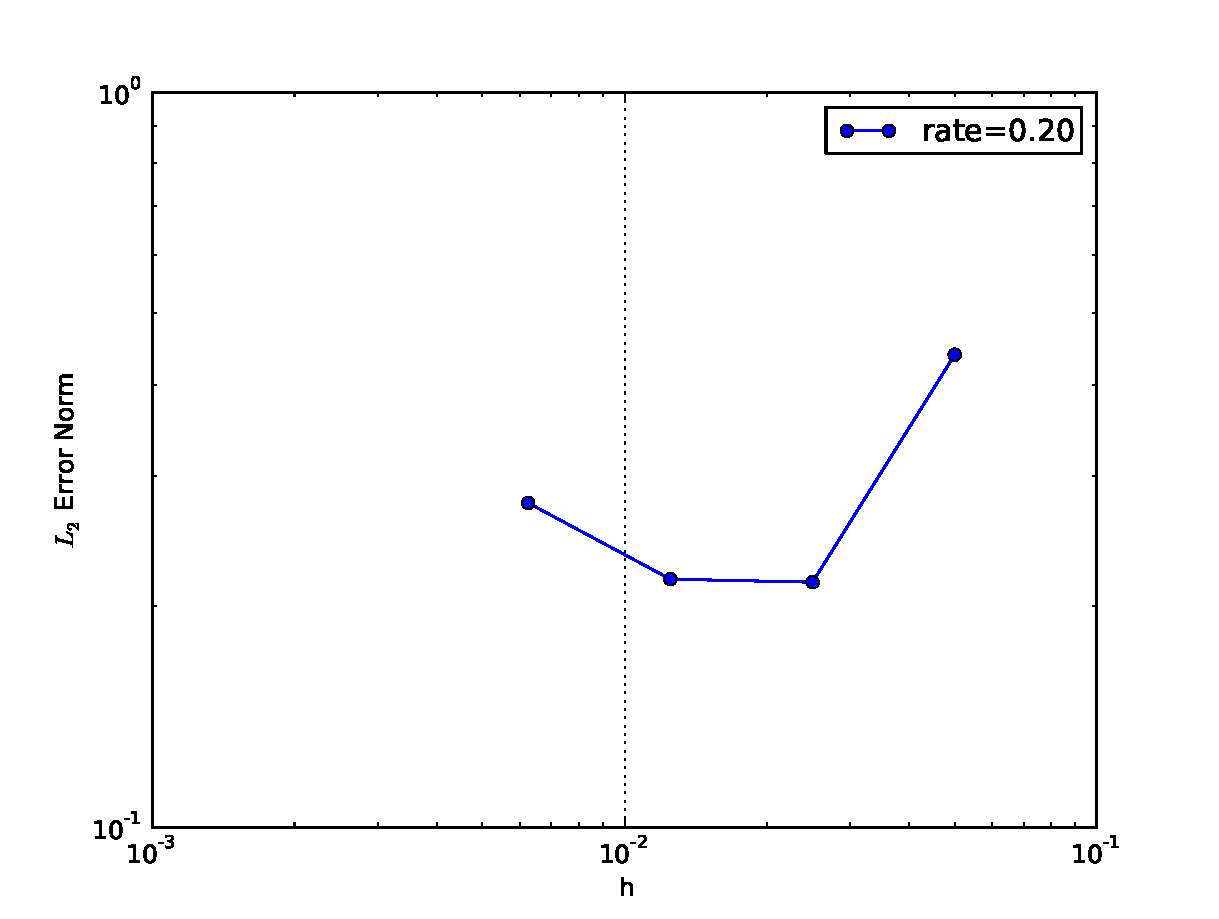
\includegraphics[width=5in]{ec-800.pdf}
\end{center}
\caption{$L_2$ convergence for $c=-800$}
\end{figure}

\begin{figure}[p]
\begin{center}
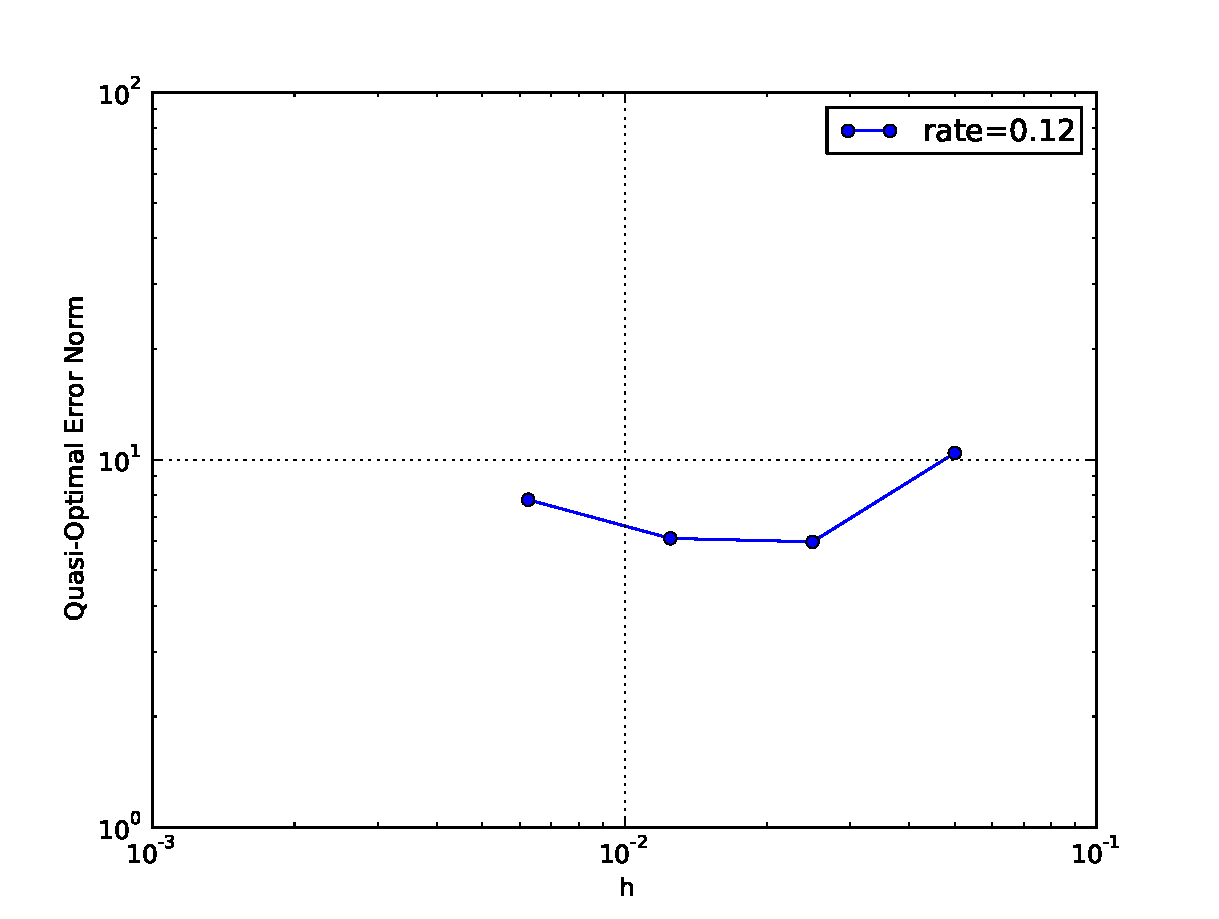
\includegraphics[width=5in]{epc-800.pdf}
\end{center}
\caption{Quasi-optimal convergence for $c=-800$}
\end{figure}

\clearpage
\newpage
\lstinputlisting[language=Python,title={FESolver.py}]{FESolver.py}

\end{document}
